%%
%% This is file `mcmthesis-demo.tex',
%% generated with the docstrip utility.
%%
%% The original source files were:
%%
%% mcmthesis.dtx  (with options: `demo')
%%
%% -----------------------------------
%%
%% This is a generated file.
%%
%% Copyright (C)
%%     2010 -- 2015 by Zhaoli Wang
%%     2014 -- 2016 by Liam Huang
%%
%% This work may be distributed and/or modified under the
%% conditions of the LaTeX Project Public License, either version 1.3
%% of this license or (at your option) any later version.
%% The latest version of this license is in
%%   http://www.latex-project.org/lppl.txt
%% and version 1.3 or later is part of all distributions of LaTeX
%% version 2005/12/01 or later.
%%
%% This work has the LPPL maintenance status `maintained'.
%%
%% The Current Maintainer of this work is Liam Huang.
%%
\documentclass{mcmthesis}
\mcmsetup{CTeX = false,   % 使用 CTeX 套装时,设置为 true
        tcn = 1920446, problem = C,
        sheet = true, titleinsheet = true, keywordsinsheet = true,
        titlepage = true, abstract = true}

\usepackage{palatino}
\usepackage{mwe}
\usepackage{graphicx}
\usepackage{subcaption}
\usepackage{float}
\usepackage{multirow}
\usepackage{indentfirst}
\usepackage{gensymb}
\usepackage[ruled,lined,commentsnumbered]{algorithm2e}
\usepackage{geometry}
% \geometry{left=2cm,right=2cm,top=2cm,bottom=2cm} %%页边距
% \usepackage{algorithm}  
\usepackage{algorithmicx}  
\usepackage{algpseudocode}  
\renewcommand{\algorithmicrequire}{\textbf{Input:}}  % Use Input in the format of Algorithm  
\renewcommand{\algorithmicensure}{\textbf{Output:}} % Use Output in the format of Algorithm 

\usepackage{minted}
\usemintedstyle{autumn}
\setminted{
    linenos,breaklines,tabsize=4,xleftmargin=1.5em,
    breaksymbol=\quad,fontfamily=courier
}

\setlength{\headheight}{14pt}
\author{}
% \usepackage{cmbright}

\begin{document}
\linespread{0.6}  %%行间距
\setlength{\parskip}{0.5\baselineskip}  %%段间距
\title{SOS: Spreading Model, Optimization, and Strategy for the Opioid Crisis}

\date{\today}
	\begin{abstract}
	As the deteriorating Opioid Crisis overwhelms the United States, the DEA/National Forensic Laboratory Information System (NFLIS) are striving to control the nationwide spread of opioid overdose indidents. In this paper, we formuate a novel framework, named \textbf{SOS ( Spreading Model, Optimization, and Strategy for the Opioid Crisis)}, seeking for new strategies to combat the exacerbating opioid crisis.
	
	Based on the report provided, we create a Spreading Model of opioid incidents, focusing on the individual counties located in five U.S. states: Ohio (OH), Kentucky (KY), West Virginia (WV), Virginia (VA), and Pennsylvania (PA). We first get the longitude and latitude of every county and utilize a \textbf{Back-Propagation Neutral Network (BPNN)} to describe the spread and characteristics of the reported opioid incidents over time. With this initial model, we can identify some possible locations where specific opioid use might have started in each of the five states.Furthermore, we analyze the U.S. Census Socio-Economic data provided with two techniques:   \textbf{Principal Component Analysis (PCA)} and \textbf{Learning Approach: Auto Encoder},  aiming to reduce the dimensions and find any important principal components. Then we make \textbf{Linear Regression (LR)} to test the validity of these components, with which we add to our Spreading Model for modification.
	
	Eventually, we identify some possible and feasible strategies for countering the opioid crisis.  After being tested by our model, these strategies are proven to be significantly effective in controlling the opioid crisis. We finally give a significant parameter bound that success is dependent upon.
	
		\begin{keywords}
		SOS; Back-Propagation Neutral Network (BPNN); Principal Component Analysis (PCA); Learning Approach: Auto Encoder;
		Linear Regression;	strategies for opioid crisis
		\end{keywords}
	\end{abstract}

\maketitle

\tableofcontents

\newpage

\section{Introduction}	
\subsection{Problem Background}
The Opioid Crisis means the rapid increase in the use of prescription and non-prescription opioid drugs in the United States beginning in the late 1990s and continuing throughout the past two decades~\cite{op}. Nowadays, it has developed into a nationwide crisis sweeping across the United States. For instance, using the data supplied with this problem, we analyze just heroin identification counts during years 2010-2017 in figure \ref{situation}, which to some extent demonstrate the rampant drug problem in these five states, especially in Ohio (OH) and Pennsylvania (PA).

\begin{figure}[htbp]
	\centering 
	\includegraphics[width=1\linewidth]{../figure/test.png}  
	\caption{Heroin identification counts in years 2010-2017 in each of the counties from five states: Ohio (OH), Kentucky (KY), West Virginia (WV), Virginia (VA), and Pennsylvania (PA)} 
	\label{situation}  
\end{figure}

Studies show that the increase in opioid overdose deaths has been dramatic, and opioids are now responsible for 49,000 of the 72,000 drug overdose deaths overall in the US in 2017~\cite{NIH}.The rate of prolonged opioid use is also increasing globally, threatening not only Americans' health but also the U.S. economy in many aspects. Consequently, president Donald Trump declared the country's opioid crisis a "national emergency"~\cite{Trump}.

Currently, the U.S. government has payed great attention and taken a bunch of measures on this issue. While the U.S. Centers for Disease Control (CDC) continue to fight the opioid overdose epidemic, simply enforcing existing laws is still a complex challenge for the Federal Bureau of Investigation (FBI), and the U.S. Drug Enforcement Administration (DEA), among others~\cite{intro}. Therefore, they need investigate the spread and characteristics of the opioids and heroin incidents in the United States, so that they can develop their strategies to better control and prevent the deteriorating opioids overdose situation.

\subsection{Our Work}
In this paper, we propose a novel framework, named SOS ( Spreading Model, Optimization, and Strategy for the Opioid Crisis), seeking for new strategies to combat the exacerbating opioid crisis. The framework of SOS is shown in Figure XXX. 

\begin{figure}[htbp]
	\centering 
	\includegraphics[width=1\linewidth]{../figure/test.png}  
	\caption{Framework of SOS: Spreading Model, Optimization, and Strategy for the Opioid Crisis} 
	\label{Framework}  
\end{figure}


We can divide our SOS framework in Figure xxx into following steps:

\begin{itemize}
\item \textbf{Spreading Model}: Based on the report provided, we focus on the individual counties located in five U.S. states: Ohio (OH), Kentucky (KY), West Virginia (WV), Virginia (VA), and Pennsylvania (PA). We first get the longitude and latitude of every county and build a \textbf{Back-Propagation Neutral Network (BPNN) Model} to describe the spread and characteristics of the reported opioid incidents over time. With this model, we identify some possible locations where specific opioid use might have started in each of the five states.
\item \textbf{Optimization}: Furthermore, we analyze the U.S. Census Socio-Economic data provided with two techniques:   \textbf{Principal Component Analysis (PCA)} and \textbf{Learning Approach: Auto Encoder} ,  aiming to reduce the dimensions and find any important principal components. Then we make \textbf{Linear Regressions} to test the validity of these components, with which we add to our Spreading Model.
\item \textbf{Strategy for the Opioid Crisis}: Eventually, we identify some possible and feasible strategies for countering the opioid crisis.  After being tested by our model, these strategies are proven to be significantly effective in controlling the opioid crisis. We finally give a significant parameter bound that success is dependent upon.
\end{itemize}

\section{Assumptions}\label{Sec-Assume}
First and foremost, we make some basic assumptions and explain their rationales.
	\paragraph{Assumption 1.}\itshape{Each state pays great attention to the drug cases and establishes common goals to overcome the opioid crisis.}
	
	\upshape This assumption is the premise of our work, because our goals as well as actions make sense only if every state strives to attack the drug problem.
	
	\paragraph{Assumption 2.}\itshape{The spread of the opioid and heroin incidents only takes place between two counties that are close to each other.}
	
	\upshape To simplify this problem, we only take short-distance spread between counties into consideration, and omit long-distance smuggling of opioid.
	
	\paragraph{Assumption 3.}\itshape{There will be no sudden enactment of strict laws or regulations on drug control.}
	
	\upshape The sudden changes of laws on drug controls will change the amount of the the cases during the period of time. There is no sign for changing of the laws, so that the assumption is reasonable. In that case, our data can be treated stable.
	
	\paragraph{Assumption 4.}\itshape{The drug identification data and the county location data are reliable to a certain extent.}
	
	\upshape Although the data can not be as complete as the fact and some statistical errors are inevitable, we make this assumption to reach one valid solution.

\section{Nomenclature}\label{Sec-Nomen}  %符号表
In this paper we use the nomenclature in Table \ref{tab:Nomen} to describe our model. Other symbols that are used only once will be described later.
\begin{table}[H]
    \centering
    \caption{Nomenclature}
    \label{tab:Nomen}
    \begin{tabular}{c|c}
\hline
    	Symbol & Definition\\
\hline
	$a_x$ & The longitude of point A\\
	$a_y$ & The latitude of point A \\
    $D_{ij}$ &  The distance between any two state counties\\
    $R^2$ & The coefficient of determination, pronounced "R squared"\\
	$h_{w}$ & A vector function depends on the input-layer weights \\
	$y$ & Target result of the function $h_{w}$ \\
	$Err_k$ & The $k$th component of the error vector $y-h_{w}$\\
	$\Delta_k$ &  A modified error $Err _{k}\times g{}'\left ( in_{k} \right )$\\
	$w_{k}$ & A set of $p$-dimensional vectors of weights or loadings\\
	$\mathbf {t} _{(i)}$ & A new $m$-dimensional vector of principal component scores \\
	$\mathbf{X^TX}$ & A positive semidefinite matrix\\
	$\mathbf{W}$ & A $p$-by-$p$ matrix whose columns are the eigenvectors of $\mathbf{X^TX}$\\
    MLP	& The Multilayer Perception\\
\hline
    \end{tabular}
\end{table}    

\section{SOS: Spreading Model, Optimization, and Strategy for the Opioid Crisis} \label{Sec-Model}
In this section, we will discuss all details about our model \textbf{SOS}. Generally, this model consists of three parts: Spreading Model  for Opioid Incidents, Optimization with Socio-Economic Components, and Strategy for the Opioid Crisis.

\subsection{Data Pre-Processing}
To begin with, we consider the relative distance between any two counties as one of the factors that affects the spreading of Opioid Crisis. However, the data of geometry information of the counties listed is not included in the dataset. Thus, we write a short python program to get the geographical locations of all the counties in the above five states from the \textbf{Microsoft Bing Map API}~\cite{bing}, which is a tool used to search through OpenStreetMap data by name and address. The official coordinates of these 462 counties that we get are partly present as follows. See \ref{code:geocode} for the complete code. 

In that case, we can calculate the distance between each two counties. The earth is a near-standard ellipsoid with an equatorial radius of 6,378.140 km and a polar radius of 6,356.755 km, with an average radius of 6,371.004 km. If we assume that the earth is a perfect sphere, then its radius is the average radius of the earth, called R. If the zero degree longitude line is the basis, the surface distance between any two points on the earth's surface can be calculated based on the longitude and latitude of the two points. Let the longitude and latitude of point $A$ be $(A_x, A_y)$, and the longitude and latitude of point $B$ be $(B_x, B_y)$. Then, according to the Trigonometric Derivation, the equation \ref{1} and equation \ref{2} for calculating the distance between two points can be obtained.

     \begin{equation}
          \label{1}
          C = \sin(A_y)*\sin(B_y)*\cos(A_x-B_x) + \cos(A_y)*\cos(B_y)
     \end{equation}
     \begin{equation}
         \label{2}
         D = R*\arccos(C)*\pi/180
     \end{equation}
    
    Using the location data we got before, we can make a matrix that represents all the distance between any two counties in these five states.
    
    Besides, we ranked the number of opioid incidents of each drug in each state county, and we get the table . Since there is no statistic significance for small amounts of data, we screened out significant data with statistically large amounts for the following modeling.
    
\subsection{ Spreading Model for Opioid Incidents }

    \subsubsection{Model Evaluation Criteria:  Coefficient of Determination}
    
    In our model, we take  Coefficient of Determination as our Evaluation Criteria.In statistics, the coefficient of determination, denoted $R^2$ or $r^2$ and pronounced "R squared", is the proportion of the variance in the dependent variable that is predictable from the independent variable(s) ~\cite{R}. 
    
    A data set has $n$ values marked $y_1$,...,$y_n$ (collectively known as $y_i$ or as a vector $y = [y_1,...,y_n]^T$), each associated with a predicted (or modeled) value $f_1$,...,$f_n$ (known as $f_i$, or sometimes $\hat{y_i}$, as a vector $f$).

   Define the residuals as $e_i = y_i$ - $f_i$ (forming a vector $\vec{e}$ ). $\bar{y}$ is the mean of the observed data: 
    $\bar{y}=\frac{1}{n}\sum_{i=1}^n y_{i}$ , then the variability of the data set can be measured using three sums of squares formulas:
    \begin{gather}
        SS_{tot}=\sum _{i} \left ( y_i-\bar{y} \right )^2\\
         SS_{reg}=\sum _{i} \left ( f_i-\bar{y} \right )^2\\
       SS_{res}=\sum _{i} \left ( y_i-f_i \right )^2=\sum _{i}e_i^2
     \end{gather}
     
    Here we use the most general definition of the coefficient of determination as equation \ref{R^2}.
    \begin{equation}\label{R^2}
        R^2\equiv 1-\frac{SS_{res}}{SS_{tot}}
    \end{equation}
   The better the linear regression fits the data in comparison to the simple average, the closer the value of $R^{2}$ is to 1. 
    
	\subsubsection{Back-Propagation Neutral Network (BPNN) Model} \label{Sec:BPNN} 
	In order to describe how the opioid identification counts spread in and between the five states, we build a Back-Propagation Neutral Network Model, using distance matrix and last year's data as input. Back-Propagation is a supervised learning algorithm, for training Artificial Neural Networks, especially,  multi-layer networks ~\cite{AI}. The weights such that the minimum error occurs is then considered to be a solution to the learning problem.
	
	Let $h_{w}$ be a vector function and $y$ be its target result. Then $Err_{k}$ be the $k$th component of the error vector $y-h_{w}$.
	
	Whereas a percentage network decomposes into $m$ seperate learning problems for an $m$-output problem, this decomposition fails in multi-layer network. The vector $h_{w}$ that returns depends on the all of the input-layer weights, so updates to those weights will depend on errors in the vector. Fortunately, this dependency is very simple in the case of any loss function that is additive across the components of the error vector $y-h_{w}$. For the $L_{2}$ loss, we have, for any weight $w$,  equation \ref{Loss}.
	\begin{equation}
	\label{Loss}
	   \frac{\partial }{\partial w}Loss\left ( w \right )=\frac{\partial }{\partial w}\left | y-h_{w}\left ( x \right ) \right |^{2}
   =\frac{\partial }{\partial w}\sum_{k}\left ( y_{k}-a_{k} \right )^{2}=\sum_{k}\frac{\partial }{\partial w}\left ( y_{k}-a_{k} \right )^{2} 
	\end{equation}

	The major complication comes from the addition of hidden layers to the network. Whereas the error ${y-h_{w}}$ at the output layer is clear, the error at the hidden layers seems mysterious because the training data do not say what value the hidden nodes should have. Fortunately, it turns out that we can back-propagate the error from the output layer to the hidden layers. The back-propagation progress emerges directly from a derivation of the overall error gradient.
	
	We can easily define a modified error $\Delta _{k}=Err _{k}\times g{}'\left ( in_{k} \right )$, where $in_{k}$ means the $k$th component of input, so that the weight update rule becomes the equation \ref{weight}.
	\begin{equation}
       \label{weight}
	    w_{j,k}\leftarrow w_{j,k}+\alpha \times a_{j} \times\Delta _{k}
	\end{equation}
	
	To update the connections between the input units and the hidden units, we need to define a quantity analogous to the error term for output nodes. Here is where we do the error back-propagation. The idea is that hidden node $j$ is ``responsible'' for some fraction of the error $\Delta _{k}$ in each of the output nodes to which it connects. Thus, the $\Delta _{k}$ values are divided according to the strength of the connections between the hidden node and the output node and are propagated back to provide the $\Delta_{j}$ values for the hidden layer. The propagation rule for the $\Delta$ values is showed in equation \ref{prop}.
	\begin{equation}
        \label{prop}
	    \Delta_{j} = g{}'\left ( in_{k} \right)\sum_{k}w_{j,k}\Delta_{k}
	\end{equation}

	Now the weight-update rule for the weights between the inputs and the hidden layer is essentially identical to the update rule for the output layer:
	\begin{equation}
	    w_{j,k}\leftarrow w_{j,k}+\alpha \times a_{j} \times\Delta _{k}
	\end{equation}
	
	The process of back-propagation can be shown as the following steps:
\begin{itemize}
\item Compute the $\Delta$ values for the output units, using the observed error.
\item Starting with output layer, repeat the following for each layer in the network, until the earliest hidden layer is reached:
\begin{itemize}
    \item[-] Propagation the $\Delta$ values back to the previous layer.
    \item[-] Update the weights between the two layers.
\end{itemize}
\end{itemize}

From above, we compute the gradient for $Loss_{k}=\left ( y_{k}-a_{k} \right )^{2}$ at the $k$th output. The gradient of this loss with respect to weights connecting the hidden layer to the output layer will be zero except for weights $w_{j,k}$ that connect to the $k$th output unit. For those weights, we have the following equation \ref{align}.

\begin{align}
\label{align}
\frac{\partial Loss_{k}}{\partial w_{j,k}}
&=-2\left ( y_{k}-a_{k} \right )\frac{\partial a_{k}}{\partial w_{j,k}}=-2\left ( y_{k}-a_{k} \right )\frac{\partial g\left ( in_{k} \right )}{\partial w_{j,k}} \notag\\
&=2\left ( y_{k}-a_{k} \right )g{}'\left ( in_{k} \right )\frac{\partial in_{k}}{\partial w_{j,k}} = 2\left ( y_{k}-a_{k} \right )g{}'\left ( in_{k} \right )\frac{\partial }{\partial w_{j,k}} \left ( \sum_{j} w_{j,k}a_{j}\right )\notag\\
&=-2\left ( y_{k}-a_{k} \right )g{}'\left ( in_{k} \right )a_{j}=-a_{j}\Delta _{k}
\end{align}

To obtain the gradient with respect to the $w_{i,j}$ weights connecting the input layer to the hidden layer, we have to expand out the activation $a_{j}$ and reapply the chain rule. We will show the derivation in gory detail because it is interesting to see how the derivation operator propagates back through the network as equation \ref{omg}.

\begin{align}
\label{omg}
\frac{\partial Loss_{k}}{\partial w_{i,j}} &=-2\left ( y_{k}-a_{k} \right )\frac{\partial a_{k}}{\partial w_{i,j}}=-2\left ( y_{k}-a_{k} \right )\frac{\partial g\left ( in_{k} \right )}{\partial w_{i,j}} \notag\\
&=-2\left ( y_{k}-a_{k} \right )g{}'\left ( in_{k} \right ) \frac{\partial in_{k}}{\partial w_{i,j}} = -2\Delta_{k}\frac{\partial }{\partial w_{i,j}} \left ( \sum_{j} w_{j,k}a_{j}\right )\notag\\ &=-2\Delta_{k}w_{j,k}\frac{\partial a_{j}}{\partial w_{i,j}}=-2\Delta_{k}w_{j,k}\frac{\partial g\left ( in_{j} \right )}{\partial w_{i,j}}=-2\Delta_{k}w_{j,k}g{}'\left ( in_{j} \right )\frac{\partial in_{j}}{\partial w_{i,j}}\notag\\ &=-2\Delta_{k}w_{j,k}g{}'\left ( in_{j} \right )\frac{\partial }{\partial w_{i,j}}\left ( \sum_{j} w_{i,j}a_{i}\right )\notag\\ 
&=-2\Delta_{k}w_{j,k}g{}'\left ( in_{j} \right )a_{i} = -a_{i}\Delta_{j}
\end{align}

 Thus, we obtain the update rules obtained earlier from intuitive considerations. It is also clear that the process can be continued for networks with more than one hidden layer.

The error value indicates how much the network's output (actual) is off the mark from the expected output (target) so that we use the \textbf{Mean Squared Error Function} to calculate the error.

In this way, we solve every individual differential to get the initial desired differential.

We just saw how back propagation of errors is used in MLP neural networks to adjust weights for the output layer to train the network. We use a similar process to adjust weights in the hidden layers of the network which we would see next with a real neural network's implementation since it will be easier to explain it with an example where we have actual numbers to play with.

   	\subsection{Optimization: Modification using Socio-economic Component}\label{Sec:Optimazation}
\subsubsection{Dimensionality Reduction}

\paragraph{\textbf{Technique 1: Principal Component Analysis (PCA)}}

~\smallskip

Now, our model can basically describe the spread and characteristics of the opioid and identify some possible locations where specific opioid use might have started. Next, we consider whether any important factors from the U.S. Census socio-economic data provided can further modify our model so that it can explain how opioid use got to its current level, what contributes to the growth in opioid addiction, and analyze who is using/abusing it despite its known dangers.

When we process the U.S. Census socio-economic data, we first adopt  the Principal component analysis (PCA), which is a statistical procedure that uses an orthogonal transformation to convert a set of observations of possibly correlated variables into a set of values of linearly uncorrelated variables called principal components. If there are $n$ observations with $p$ variables, then the number of distinct principal components is $\min(n-1,p)$. 

PCA is mathematically defined as an orthogonal linear transformation that transforms the data to a new coordinate system such that the greatest variance by some projection of the data comes to lie on the first coordinate (called the first principal component), the second greatest variance on the second coordinate, and so on.

Consider a data matrix, $\mathbf{X}$, with column-wise zero empirical mean (the sample mean of each column has been shifted to zero), where each of the n rows represents a different repetition of the experiment, and each of the p columns gives a particular kind of feature (say, the results from a particular sensor).

Mathematically, the transformation is defined by a set of p-dimensional vectors of weights or loadings $ \mathbf {w} _{(k)}=(w_{1},\dots ,w_{p})_{(k)}$ that map each row vector $\mathbf{x}_{(i)}$ of X to a new vector of principal component scores $ \mathbf {t} _{(i)}=(t_{1},\dots ,t_{m})_{(i)}$, given by
$$ {t_{k}}_{(i)}=\mathbf {x} _{(i)}\cdot \mathbf {w} _{(k)}\qquad \mathrm {for} \qquad i=1,\dots ,n\qquad k=1,\dots ,m$$
in such a way that the individual variables $ t_{1},\dots ,t_{m}$ of t considered over the data set successively inherit the maximum possible variance from $\mathbf {x}$, with each loading vector $\mathbf {w}$ constrained to be a unit vector. \\

In order to maximize variance, the first loading vector $\mathbf{w}_{(1)}$ thus has to satisfy
\begin{equation}
    \mathbf {w} _{(1)}={\underset {\Vert \mathbf {w} \Vert =1}{\operatorname {\arg \,max} }}\,\left\{\sum _{i}\left(t_{1}\right)_{(i)}^{2}\right\}={\underset {\Vert \mathbf {w} \Vert =1}{\operatorname {\arg \,max} }}\,\left\{\sum _{i}\left(\mathbf {x} _{(i)}\cdot \mathbf {w} \right)^{2}\right\}
\end{equation}
Equivalently, writing this in matrix form gives
\begin{equation}
    \mathbf {w} _{(1)}={\underset {\Vert \mathbf {w} \Vert =1}{\operatorname {\arg \,max} }}\,\{\Vert \mathbf {Xw} \Vert ^{2}\}={\underset {\Vert \mathbf {w} \Vert =1}{\operatorname {\arg \,max} }}\,\left\{\mathbf {w} ^{T}\mathbf {X} ^{T}\mathbf {Xw} \right\}
\end{equation} 

Since $\mathbf{w}_{(1)}$ has been defined to be a unit vector, it equivalently also satisfies
\begin{equation}
    \mathbf {w} _{(1)}={\operatorname {\arg \,max} }\,\left\{{\frac {\mathbf {w} ^{T}\mathbf {X} ^{T}\mathbf {Xw} }{\mathbf {w} ^{T}\mathbf {w} }}\right\}
\end{equation}

The quantity to be maximised can be recognised as a Rayleigh quotient. A standard result for a positive semidefinite matrix such as $\mathbf{X^TX}$ is that the quotient's maximum possible value is the largest eigenvalue of the matrix, which occurs when w is the corresponding eigenvector.

With $\mathbf{w}_{(1)}$ found, the first principal component of a data vector $\mathbf{x}_{(1)}$ can then be given as a score $t_{1(1)} = \mathbf{x}_{(1)} \cdot \mathbf{w}_{(1)}$ in the transformed co-ordinates, or as the corresponding vector in the original variables, $\{\mathbf{x}_{(1)} \cdot \mathbf{w}_{(1)}\} \mathbf{w}_{(1)}$. \\

The $k$th component can be found by subtracting the first $k_1$ principal components from $\textbf{X}$:
\begin{equation}
    \mathbf {\hat {X}} _{k}=\mathbf {X} -\sum _{s=1}^{k-1}\mathbf {X} \mathbf {w} _{(s)}\mathbf {w} _{(s)}^{\rm {T}}
\end{equation}

and then finding the loading vector which extracts the maximum variance from this new data matrix
\begin{equation}
    \mathbf {w} _{(k)}={\underset {\Vert \mathbf {w} \Vert =1}{\operatorname {arg\,max} }}\left\{\Vert \mathbf {\hat {X}} _{k}\mathbf {w} \Vert ^{2}\right\}={\operatorname {\arg \,max} }\,\left\{{\tfrac {\mathbf {w} ^{T}\mathbf {\hat {X}} _{k}^{T}\mathbf {\hat {X}} _{k}\mathbf {w} }{\mathbf {w} ^{T}\mathbf {w} }}\right\}
\end{equation}

It turns out that this gives the remaining eigenvectors of $\mathbf{X^TX}$, with the maximum values for the quantity in brackets given by their corresponding eigenvalues. Thus the loading vectors are eigenvectors of $\mathbf{X^TX}$.

The $k$th principal component of a data vector $\mathbf{x}_{(i)}$ can therefore be given as a score $t_{k(i)} = \mathbf{x}_{(i)} \cdot \mathbf{w}_{(k)}$ in the transformed co-ordinates, or as the corresponding vector in the space of the original variables, $\{\mathbf{x}_{(i)} \cdot \mathbf{w}_{(k)}\} \mathbf{w}_{(k)}$, where $\mathbf{w}_{(k)}$ is the $k$th eigenvector of $\mathbf{X^TX}$.

The full principal components decomposition of $\mathbf{X}$ can therefore be given as
\begin{equation}
    \mathbf {T} =\mathbf {X} \mathbf {W}
\end{equation}

where $\mathbf{W}$ is a $p$-by-$p$ matrix whose columns are the eigenvectors of $\mathbf{X^TX}$. The transpose of $\mathbf{W}$ is sometimes called the whitening or sphering transformation. 

\paragraph{\textbf{Technique 2: Deep Learning Approach: Auto Encoder}}

~\smallskip

An autoencoder is an artificial neural network used for unsupervised learning of efficient codings. The aim of an autoencoder is to learn a representation (encoding) for a set of data, typically for the purpose of dimensionality reduction. Recently, the autoencoder concept has become more widely used for learning generative models of data. Some of the most powerful AI in the 2010s involves stacking sparse autoencoders in a deep learning network.

Architecturally, the simplest form of an autoencoder is a feedforward, non-recurrent neural network very similar to the multilayer perception (MLP), having an input layer, an output layer and one or more hidden layers connecting them, but with the output layer having the same number of nodes as the input layer, and with the purpose of reconstructing its own inputs (instead of predicting the target value $Y$ given inputs $X$. Therefore, autoencoders are unsupervised learning models.

An autoencoder always consists of two parts, the encoder and the decoder, which can be defined as transitions $\phi$  and $\psi$ such that:
\begin{gather}
\phi :{\mathcal {X}}\rightarrow {\mathcal {F}} \notag\\
\psi :{\mathcal {F}}\rightarrow {\mathcal {X}} \notag\\
\phi ,\psi ={\underset {\phi ,\psi }{\operatorname {arg\,min} }}\,\|X-(\psi \circ \phi )X\|^{2}
\end{gather}

In the simplest case, where there is one hidden layer, the encoder stage of an autoencoder takes the input $\mathbf {x} \in \mathbb {R} ^{d}={\mathcal {X}}$ and maps it to $\mathbf {z} \in \mathbb {R} ^{p}={\mathcal {F}}$:
\begin{equation}
    \mathbf {z} =\sigma (\mathbf {Wx} +\mathbf {b} )
\end{equation}

This image $\mathbf {z}$  is usually referred to as code, latent variables, or latent representation. Here, $\sigma$  is an element-wise activation function such as a sigmoid function or a rectified linear unit. $\mathbf {W}$  is a weight matrix and $\mathbf {b}$  is a bias vector. After that, the decoder stage of the autoencoder maps $\mathbf {z}$  to the reconstruction $\mathbf {x'}$  of the same shape as $\mathbf {x}$ :
\begin{equation}
    \mathbf {x'} =\sigma '(\mathbf {W'z} +\mathbf {b'} )
\end{equation}


where $ \mathbf {\sigma '} ,\mathbf {W'} ,{\text{ and }}\mathbf {b'} $ for the decoder may differ in general from the corresponding $ \mathbf {\sigma } ,\mathbf {W} ,{\text{ and }}\mathbf {b} $ for the encoder, depending on the design of the autoencoder.

Autoencoders are also trained to minimise reconstruction errors (such as squared errors):
\begin{equation}
     {\mathcal {L}}(\mathbf {x} ,\mathbf {x'} )=\|\mathbf {x} -\mathbf {x'} \|^{2}=\|\mathbf {x} -\sigma '(\mathbf {W'} (\sigma (\mathbf {Wx} +\mathbf {b} ))+\mathbf {b'} )\|^{2}
\end{equation}

where $\mathbf {x}$  is usually averaged over some input training set.

If the feature space $\mathcal {F}$ has lower dimensionality than the input space $\mathcal {X}$, then the feature vector $\phi (x)$ can be regarded as a compressed representation of the input $x$. If the hidden layers are larger than the input layer, an autoencoder can potentially learn the identity function and become useless. However, experimental results have shown that autoencoders might still learn useful features in these cases.

\subsubsection{Linear Regression (LR) for Principle Component}
After we choose the number of components to express the use or trends-in-use according to the U.S. Census socio-economic data, we apply linear regression to test if the components we choose can give a satisfying result that is close to the reports given by the NFLIS data. In this way, we can a score of this linear regression. The closer it approaches $1$, the better the components show the fact.

Given a data set $\left \{ y_{i}, x_{i1}, \cdots , x_{ip} \right \}_{i = 1}^{n}$ of n statistical units, a linear regression model assumes that the relationship between the dependent variable $y$ and the $p$-vector of regressors $x$ is linear. This relationship is modeled through a disturbance term or error variable $ε$ , an unobserved random variable that adds "noise" to the linear relationship between the dependent variable and regressors. Thus the model takes the form  as the following shows.

\begin{equation}
    y_i = \beta_{0}1+ \beta_{1}x_{i1}+\cdots +\beta_{p}x_{ip} + \varepsilon _{i} = x_{i}^{T}\beta + \varepsilon_{i}
\end{equation}

The superscript $T$ denotes the transpose, so that $x_{i}^{T}\beta$ is the inner product between vectrs $x_{i}$ and $\beta$. 

Often these n equations are stacked together and written in matrix notation as the following.

\begin{equation}
    y = X\beta + \varepsilon
\end{equation}

\begin{itemize}
\item[-] $y$ is a vector of observed values $y_{i} ( i = 1, \cdots, n )$ of the variable called the regressand, endogenous variable, response variable, measured variable, criterion variable, or dependent variable. This variable is also sometimes known as the predicted variable. $X$ may be seen as a matrix of row-vectors 
\item[-] $x_{i}$ or of n-dimensional column-vectors $X_{j}$, which are known as regressors, exogenous variables, explanatory variables, covariates, input variables, predictor variables, or independent variables (not to be confused with the concept of independent random variables).
 \item[-] $\beta$ is a $( p + 1 )$-dimensional parameter vector, where $\beta _{0}$ is the intercept term (if one is included in the model—otherwise $\beta$ is $p$-dimensional). Its elements are known as effects or regression coefficients (although the latter term is sometimes reserved for the estimated effects).
\item[-] $\varepsilon$ is a vector of values $\varepsilon _{i}$. This part of the model is called the error term, disturbance term, or sometimes noise (in contrast with the "signal" provided by the rest of the model).

\end{itemize}

\subsubsection{Results for Dimension Reduction and Linear Regression}

We have selected the most important factors from the $596$ dimensions that the U.S. Census socio-economic data provides by dimensionality reduction. And then, we use linear regression to test our selection and get the score for each selection. In this way, we can get a satisfying set of components. 

According to PCA, we can get the variance ratio, which shows the ratio of the variance value of each principal component to the total variance value after dimension reduction. The larger the value of the variance ratio, the more important the principal component.

According to LR, we can get a score for the fitting. Actually, the score is the $R^{2}$ of linear regression results and the fact data from the NFLIS Data, which shows how closer the results we get from the components reach the fact. The closer it approaches $1$, the better the components can express the fact.

In addition, to get a good result, we also need to select the way how to deal with the data given by the U.S. Census socio-economic data. So we apply the PCA as well as LR to the these data in four ways, and show the results by diagrams:

\begin{itemize}
    \item Analyze all the data over the years ranging from 2010 to 2016 of the five states respectively, and the results are shown in figure \ref{fig:pca_state}.
    \begin{figure}[H]
    \centering
    \begin{subfigure}[b]{0.49\textwidth}
        \includegraphics[width=\textwidth]{../figure/pca_state_ratio.eps}
        \subcaption{The ratio of data retained after dimensionality reduction among five states in 2010-2016 against different components}
        \label{fig:pca_state_ratio}
    \end{subfigure}
    \begin{subfigure}[b]{0.49\textwidth}
        \includegraphics[width=\textwidth]{../figure/pca_state_score.eps}
        \subcaption{The $R^2$ of linear regression results among five states in 2010-2016 against different components }
        \label{fig:pca_state_score}
    \end{subfigure}
    \caption{PCA and LR results of data among five states in 2010-2016 against different components}\label{fig:pca_state}
\end{figure}

We can see when we choose 4 components to describe this problem, the explained variance ratio almost reaches 1. That is to say that 

    \item Analyze the data of 2010 of the five states respectively, and the results are shown in figure \ref{fig:pca_state_2010}.
    \begin{figure}[H]
    \centering
    \begin{subfigure}[b]{0.49\textwidth}
        \includegraphics[width=\textwidth]{../figure/pca_state_2010_ratio.eps}
        \subcaption{The ratio of data retained after dimensionality reduction among five states in 2010 against different components}
        \label{fig:pca_state_2010_ratio}
    \end{subfigure}
    \begin{subfigure}[b]{0.49\textwidth}
        \includegraphics[width=\textwidth]{../figure/pca_state_2010_score.eps}
        \subcaption{The $R^2$ of Linear Regression results among five states in 2010 against different components}
        \label{fig:pca_state_2010_score}
    \end{subfigure}
    \caption{PCA and LR results of data among five states in 2010 against different components}\label{fig:pca_state_2010}
\end{figure}

    \item Analyze the data of all the five states of 2010 to 2016 respectively, and the results are shown in figure \ref{fig:pca_year}.
    \begin{figure}[H]
    \centering
    \begin{subfigure}[b]{0.49\textwidth}
        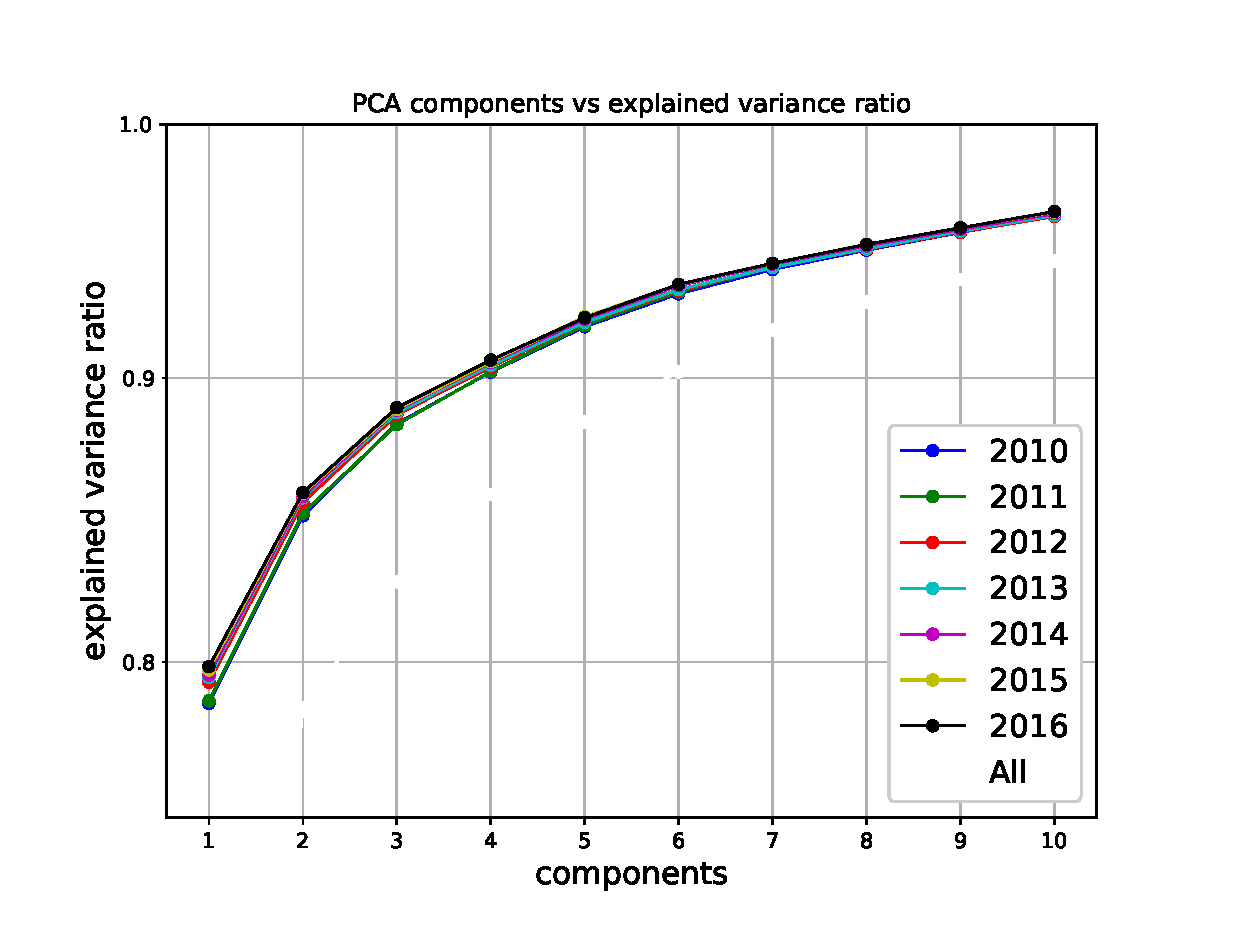
\includegraphics[width=\textwidth]{../figure/pca_year_ratio.eps}
        \subcaption{The ratio of data remained after dimensionality reduction in 2010-2017}
        \label{fig:pca_year_ratio}
    \end{subfigure}
    \begin{subfigure}[b]{0.49\textwidth}
        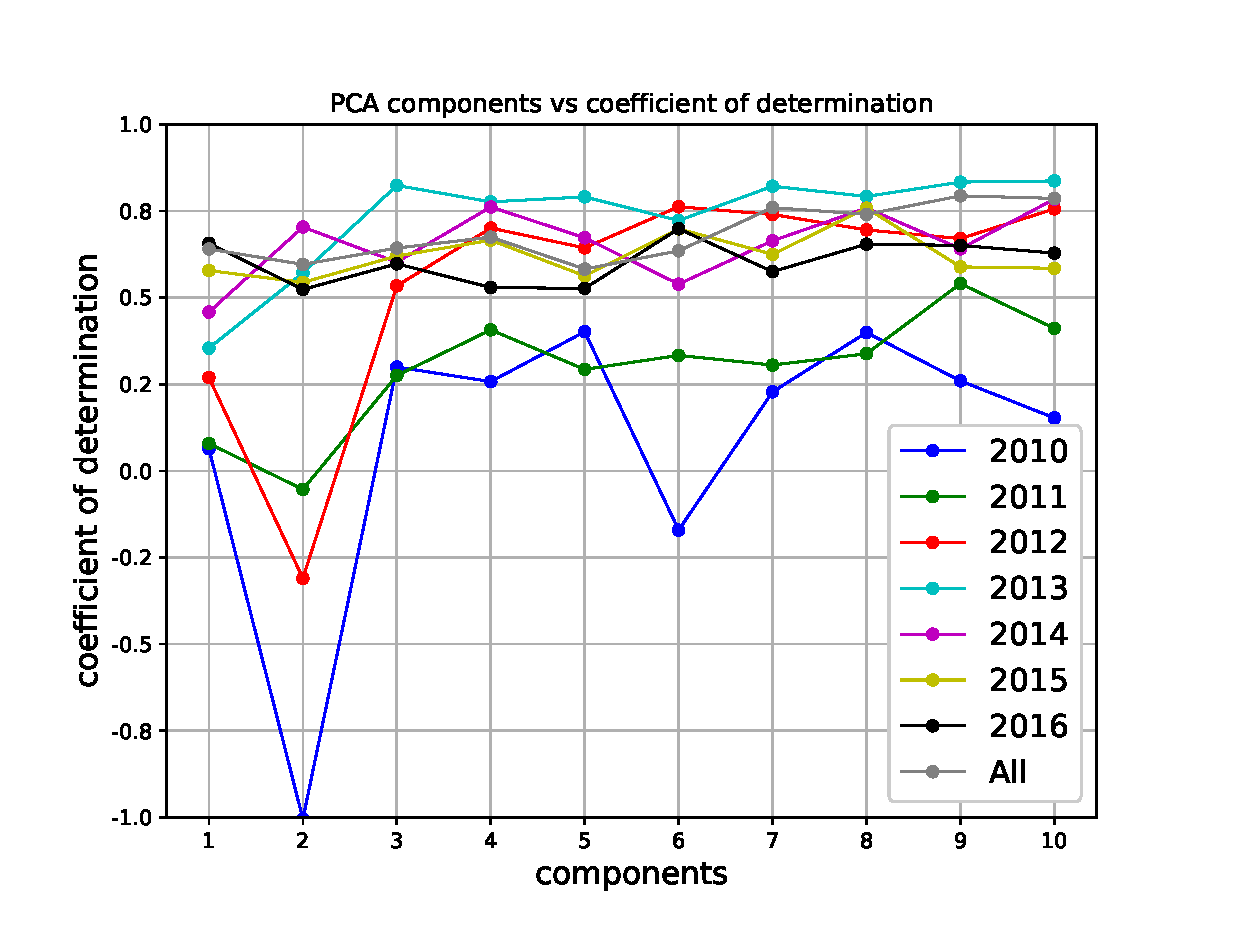
\includegraphics[width=\textwidth]{../figure/pca_year_score.eps}
        \subcaption{The $R^2$ of Linear Regression results of data in 2010-2017 against different aggregations}
        \label{fig:pca_year_score}
    \end{subfigure}
    \caption{PCA and LR results of data in 2010-2017 against different aggregations}\label{fig:pca_year}
\end{figure}

    \item Analyze the data of the state PA of 2010 to 2016 respectively, and the results are shown in figure \ref{fig:pca_year_PA}.
    \begin{figure}[H]
    \centering
    \begin{subfigure}[b]{0.49\textwidth}
        \includegraphics[width=\textwidth]{../figure/pca_year_PA_ratio.eps}
        \subcaption{The ratio of data after dimensionality reduction in PA in 2010-2017}
        \label{fig:pca_year_PA_ratio}
    \end{subfigure}
    \begin{subfigure}[b]{0.49\textwidth}
        \includegraphics[width=\textwidth]{../figure/pca_year_PA_score.eps}
        \subcaption{The $R^2$ of Linear Regression results in PA over years against different aggregations}
        \label{fig:pca_year_PA_score}
    \end{subfigure}
    \caption{PCA and LR results of data in PA in 2010-2017 against different aggregations}\label{fig:pca_year_PA}
\end{figure}
\end{itemize}

From the visualization that we have shown above, we can see 

We take the U.S. Census socio-economic data of KY state ranging from 2010 to 2016 as an example.

In PCA, we choose to reduce the dimensions to four because the variance ratio reaches a threshold of about $0.01$ after that. The variance ratios are 
\begin{center}
    $0.59396827$, $0.28748557$, $0.02754973$, $0.02732665$.
\end{center}

From these four dimension, we can get the score of about $0.92$ by linear regression, which shows a good result of the dimension reduction. 

As we mentioned before, the five states can be treated similar. So we can apply the same method to these states and combine the results for all five states. The results are shown below: 


	\subsection{Strategy for the Opioid Crisis}\label{Sec:Strategy}
	
	Understanding that certain levels of drug use are inevitable, so we should focus on minimizing adverse effects associated with drug use rather than stopping the behavior itself. In the context of the opioid epidemic, we propose the \textbf{Harm Reduction Strategies} that are designed to improve health outcomes and reduce overdose deaths.
	
    It can be divided into three aspects:
\paragraph{\textbf{Supply Control}}

~\smallskip

\begin{itemize}
    \item Requiring manufacturers of long-acting opioids to sponsor educational programs for prescribers. Through these educational programs, we can control opioid supply and help deter off-label and over-prescribing, making a threshold to those who want to abuse the opioids.
    \item We need to strengthen cooperation with countries such as Colombia and Mexico, to crack down on cross-border drug crimes.
\end{itemize}

\paragraph{\textbf{Spread Control}}

~\smallskip

\begin{itemize}
    \item Strengthen public health data reporting and collection to improve the timeliness and specificity of data and to inform a real-time public health response as the opioid epidemic evolves,so that our Spreading Model can forecast the opioid epidemic more precisely.
    \item Strengthening Public Health Data and Reporting. Timely, high-quality data help both public health officials and law enforcement understand the extent of the problem and how it is evolving, develop interventions, focus resources where they are needed most, and evaluate the success of prevention and response efforts. 
\end{itemize}

\paragraph{\textbf{Demand Control}}

~\smallskip

\begin{itemize}
    \item Advance the practice of pain management to enable access to high-quality, evidence-based pain care that reduces the burden of pain for individuals, families, and society while also reducing the inappropriate use of opioids and opioid-related harms. Only by making opioid control and management more rigorous and formal can we effectively combat illicit drug abuse.
\end{itemize}


\section{Model Analysis}\label{Sec-Analysis}

\subsection{Sensitivity Analysis}

\subsection{Strengths and Weaknesses}
\subsubsection{Strengths}
\begin{itemize}
\item \textbf{}
\item \textbf{}
\end{itemize}


\subsubsection{Weaknesses}
\begin{itemize}
\item \textbf{No Verification of Raw Data:} We have no guarantee of the accuracy of given data , and the data is not complete.
\item \textbf{No Involvement of Other States:} We do not consider states other than OH, KY, WV, VA, and PA, due to the lack of relevant data.
\item \textbf{No Accurate Geographical Information: } We use the the official coordinates of counties to represent its geographical location. And we have no guarantee of the accuracy of the data  from the Search (Nominatim) API~\cite{NO}.
\end{itemize}


\section{Conclusion} \label{Sec-Conclusion}
In this paper,we propose a novel framework called \textbf{SOS} (Spreading Model, Optimization, and Strategy for the Opioid Crisis). First we create a \textbf{Back-Propagation Neutral Network  (BPNN) Model} to describe the spread and characteristics of the opioid incidents in and between the five states over time. With this model we identified possible locations where specific opioid use might have emerged in each of the five states. Second we adopt two different techniques: \textbf{Principal Component Analysis (PCA)} and \textbf{Learning Approach: Auto Encoder}, to extract principal components from the U.S. Census Socio-Economic data. After testing the validity of these component with \textbf{Linear Regression} ,  we add to our Spreading Model for modification. Third we identify possible strategies for countering the opioid crisis. After being tested by our model, these strategies are proven to be significantly effective in controlling the opioid crisis, and we give a significant parameter bound that success is dependent upon. Finally, we conduct sensitivity analysis of some parameters in our model and discuss the strengths and weakness of our work.

\newpage
\section*{MEMORANDUM} 

\noindent\textbf{To:} Chief Administrator, DEA/NFLIS Database

\noindent\textbf{From:} Team \# 1920446

\noindent\textbf{Date}: Jananry 29, 2019

\noindent\textbf{Subject:}

Honorable Chief Administrator, DEA/NFLIS Database,


\addcontentsline{toc}{section}{MEMORANDUM}

\subsection*{Part 1:  }
\addcontentsline{toc}{subsection}{Part 1: }

\paragraph{one}

\paragraph{two}

\paragraph{three}

\subsection*{Part 2: }
\addcontentsline{toc}{subsection}{Part 2: }

\paragraph{one}

\paragraph{two}

\paragraph{three}

\subsection*{Part 3: Strategies}
\addcontentsline{toc}{subsection}{Part 3: }


The above is the summary of our study. We sincerely hope that it will provide you with useful information.

Thanks!

\newpage

\bibliographystyle{IEEEtran}
\bibliography{newrefs}
	
\ \newpage

\begin{appendices}

\section{Python Code}

\subsection{geocode.py}\label{code:geocode}
\inputminted{python}{../src/geocode.py}

\section{2}

\end{appendices}
\end{document}

%%
%% This work consists of these files mcmthesis.dtx,
%%                                   figures/ and
%%                                   code/,
%% and the derived files             mcmthesis.cls,
%%                                   mcmthesis-demo.tex,
%%                                   README,
%%                                   LICENSE,
%%                                   mcmthesis.pdf and
%%                                   mcmthesis-demo.pdf.
%%
%% End of file `mcmthesis-demo.tex'.
